\section{Diagramma delle classi}
\index{Diagramma delle classi}

Nella sezione seguente verranno descritte nel dettaglio le classi che formeranno la struttura del sistema attraverso il diagramma delle classi.\\
Saranno quindi descritte, oltre alle classi, anche tutte le relazioni che intercorrono tra di esse e i ruoli dei gestori.\\

\subsection{Utente Autenticabile}
\index{Utente Autenticabile}

\begin{figure}[htbp]
    \centering
    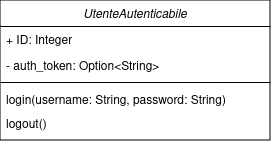
\includegraphics[width=0.25\textwidth]{Images/UtenteAutenticabile-Class.png}
    \caption{Classe Utente Autenticabile}
    \label{fig:UtenteAutenticabile}
\end{figure}

Questa classe rappresenta la figura dell'utente che utilizza l'applciazione mobile.\\
Gli utenti hanno accesso a tutte le funzionalità del sistema anche se non autenticati, quindi questa classe rappresenta tutti gli utenti che utilizzano l'applicazione e hanno le capabilities per eseguire l'accesso al sistema.\\

\textbf{Attributi:}\\

Gli attributi che caratterizzano questa classe sono:
\begin{itemize}
    \item \textbf{ID}: Attributo che rappresenta univocamente l'utente non autenticato.
    \item \textbf{auth\_token}: Attributo che rappresenta il token di autenticazione dell'utente. E' impostato ad opzionale, in quanto se l'utente non ha eseguto l'accesso questo parametro risulterà vuoto.
\end{itemize}
 
\textbf{Metodi:}\\

I metodi a disposizione della classe sono:
\begin{itemize}
    \item \textbf{login(username, password)}: Metodo utilizzato per effettuare il login all'interno dell'applicazione. Utilizzando questo metodo l'utente diventa un "Utente autenticato".\\Sono utilizzati metodi del gestore "Gestione utente" e del gestore "Gestione autenticazione" per effettuare il login.
    \item \textbf{logout()}: Metodo utilizzato per effettuare il logout dall'applicazione, cosi' da disconnettere l'utente dal servizio.\\
\end{itemize} 

\clearpage

\subsection{Utente}
\index{Utente}

\begin{figure}[htbp]
    \centering
    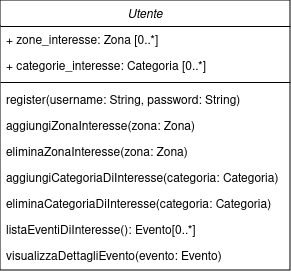
\includegraphics[width=0.25\textwidth]{Images/Utente-Class.png}
    \caption{Classe Utente}
    \label{fig:utente}
\end{figure}

La classe in questione deriva dalla classe precedente (Classe Utente, figura \ref{fig:utente}) e rappresenta tutti gli utenti che andranno ad utilizzare l'applicativo mobile.\\
Possono aver eseguito la fase di login come no, in quanto in ogni caso è garantito loro l'accesso completo alle funzionalità disponibili.\\

\textbf{Attributi:}\\
Sono a disposizione quelli della classe Utente (Figura \ref{fig:utente}), con l'aggiunta di:
\begin{itemize}
    \item \textbf{zone\_interesse}: Attributo che rappresenta le zone di interesse impostate dall'utente.
    \item \textbf{categorie\_interesse}: Attributo che rappresenta le categorie di interesse impostate dall'utente.\\
\end{itemize}

\textbf{Metodi:}\\
Anche i metodi sono gli stessi a disposizione dell'utente non autenticato, aggiungendo però il metodo:
\begin{itemize}
    \item \textbf{register(username, password)}: Metodo che permette all'utente di registrarsi per la prima volta all'interno dell'applicazione.\\Sono utilizzati metodi del gestore "Gestione utente" e del gestore "Gestione autenticazione" per effettuare la registrazione. Anche questo metodo fa diventare l'utente un "Utente autenticato".
    \item \textbf{gestioneZoneInteresse(zona)}: Metodo che permette all'utente di gestire le sue zone di interesse.
    \item \textbf{gestioneCategorieInteresse(categoria)}: Metodo che permette all'utente di gestire le sue categorie di interesse.
    \item \textbf{listaEventi()}: Metodo che permette all'utente di visualizzare la lista di tutti gli eventi presenti nel sistema.
    \item \textbf{visualizzaDettagliEvento(evento)}: Metodo che permette all'utente di visualizzare i dettagli di un singolo evento.
\end{itemize}

\clearpage

\subsection{Utente amministratore}
\index{Utente amministratore}

\begin{figure}[htbp]
    \centering
    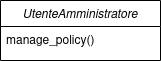
\includegraphics[width=0.25\textwidth]{Images/UtenteAmministratore-Class.png}
    \caption{Classe Utente Amministratore}
    \label{fig:utente_amministratore}
\end{figure}

La classe utente amministratore deriva dalla classe Utente Autenticabile (Figura \ref{fig:UtenteAutenticabile}) e rappresenta quell'utente con i permessi per gestire l'intero sistema.\\

Non vengono aggiunti nuovi attributi, in quanto quelli derivati dalla classe Utente Autenticabile sono sufficienti per rappresentare l'utente amministratore.\\

\textbf{Metodi:}\\
I metodi a disposizione della classe sono:

\begin{itemize}
    \item \textbf{managePolicy()}: Metodo che permette all'utente amministratore di gestire le policy del sistema.
\end{itemize}

\subsection{Utente autorizzato}
\index{Utente autorizzato}

\begin{figure}[htbp]
    \centering
    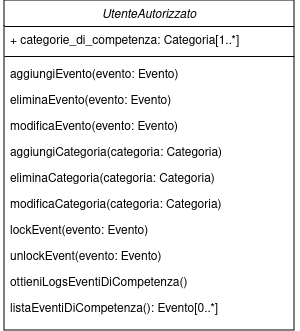
\includegraphics[width=0.3\textwidth]{Images/UtenteAutorizzato-Class.png}
    \caption{Classe Utente Autorizzato}
    \label{fig:utente_autorizzato}
\end{figure}

La classe Utente Autorizzato, anch'essa derivata da Utente Autenticabile (Figura \ref{fig:UtenteAutenticabile}) rappresenta tutti gli utenti autorizzati dal comune di Trento a pubblicare eventi e criticità a sistema.\\

\textbf{Attributi:}\\
Gli attributi che definiscono questa classe sono, oltre a quelli derivati dalla classe Utente Autenticabile, i seguenti:
\begin{itemize}
    \item \textbf{categorie\_di\_competenza}: Riporta le categorie su cui l'utente ha competenza.\\
\end{itemize}

\textbf{Metodi:}\\
I metodi a disposizione della classe sono:
\begin{itemize}
    \item \textbf{aggiungiEvento(evento)}: Metodo che permette all'utente autorizzato di creare ed aggiungere un evento al sistema.
    \item \textbf{modificaEvento(evento)}: Metodo che permette all'utente autorizzato di modificare ed aggiornare un evento precedentemente creato.
    \item \textbf{eliminaEvento(evento)}: Metodo che permette all'utente autorizzato di eliminare dal sistema un evento precedentemente creato.
    \item \textbf{aggiungiCategoria(categoria)}: Metodo che permette all'utente autorizzato di creare ed aggiungere una sottocategoria di eventi al sistema.
    \item \textbf{modificaCategoria(categoria)}: Metodo che permette all'utente autorizzato di modificare ed aggiornare una sottocategoria di eventi precedentemente creata.
    \item \textbf{eliminaCategoria(categoria)}: Metodo che permette all'utente autorizzato di eliminare dal sistema una sottocategoria di eventi precedentemente creata.
    \item \textbf{lockEvento(evento)}: Metodo che permette all'utente autorizzato di bloccare un evento per evitare che venga modificato da altri utenti (Mutua esclusione).
    \item \textbf{unlockEvento(evento)}: Metodo che permette all'utente autorizzato di sbloccare un evento precedentemente bloccato.
    \item \textbf{ottieniLogEventiDiCompetenza()}: Metodo che permette all'utente autorizzato di ottenere il log di tutti gli eventi di sua competenza.
    \item \textbf{listaEventiDiCompetenza()}: Metodo che permette all'utente autorizzato di visualizzare la lista di tutti gli eventi di sua competenza presenti nel sistema.
\end{itemize}

\clearpage

\subsection{Evento}
\index{Evento}

\begin{figure}[htbp]
    \centering
    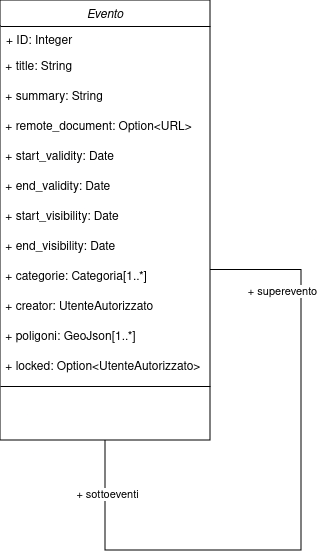
\includegraphics[width=0.25\textwidth]{Images/Evento-Class.png}
    \caption{Classe Evento}
    \label{fig:evento}
\end{figure}

La classe "Evento" rappresenta un evento o criticita' che l'utente amministratore pubblica sul sistema e che e' possibile visualizzare da applicativo mobile.

\textbf{Attributi:}\\
\begin{itemize}
    \item \textbf{ID}: Attributo che identifica univocamente l'evento pubblicato sul sistema.
    \item \textbf{title}: Attributo che rappresenta il titolo dell'evento.
    \item \textbf{summary}: Attributo che rappresenta la descrizione dell'evento.
    \item \textbf{start\_validity}: Attributo che riporta la data d'inizio validità dell'evento.
    \item \textbf{end\_validity}: Attributo che riporta la data di fine validità dell'evento.
    \item \textbf{start\_visibility}: Attributo che riporta la data d'inizio visibilità dell'evento.
    \item \textbf{end\_visibility}: Attributo che riporta la data di fine visibilità dell'evento.
    \item \textbf{categorie}: Attributo che rappresenta la categoria a cui l'evento appartiene.
    \item \textbf{sottoeventi}: Attributo che rappresenta tutti i sottoeventi che compongono l'evento stesso.
    \item \textbf{creator}: Attributo che rappresenta l'utente autorizzato che ha creato l'evento.
    \item \textbf{poligoni}: Attributo che rappresenta i poligoni che delimitano l'evento.
    \item \textbf{locked}: Attributo che rappresenta lo stato di blocco dell'evento.
\end{itemize}

Per la classe in questione non sono previsti metodi.

\clearpage 

\subsubsection{Zona}
\index{Zona}

\begin{figure}[htbp]
    \centering
    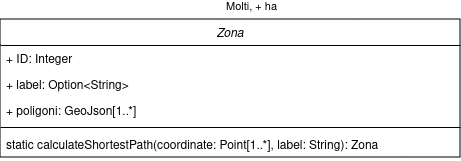
\includegraphics[width=0.5\textwidth]{Images/Zona-Class.png}
    \caption{Classe Zona d'interesse}
    \label{fig:zona}
\end{figure}

Questa classe rappresenta tutte le zone o i percorsi che risultano d'interesse per l'utente.\\

\textbf{Attributi:}\\
Gli attributi che caratterizzano questa classe sono:
\begin{itemize}
    \item \textbf{ID}: Attributo che identifica univocamente la zona d'interesse o il percorso richiesto dall'utente.
    \item \textbf{label}: Attributo che rappresenta il nome della zona d'interesse o del percorso.
    \item \textbf{poligoni}: Attributo che rappresenta i poligoni che delimitano la zona d'interesse o che disegnano il percorso.\\
\end{itemize}

\textbf{Metodi:}\\
Il metodo a disposizione della classe è:
\begin{itemize}
    \item \textbf{calculateShortestPath(coordinate)}: Metodo invocato per eseguire il calcolo del percorso più breve evitando tutte le criticita' presenti sulla mappa.
\end{itemize}

\clearpage

\subsubsection{Categoria}
\index{Categoria}

\begin{figure}[htbp]
    \centering
    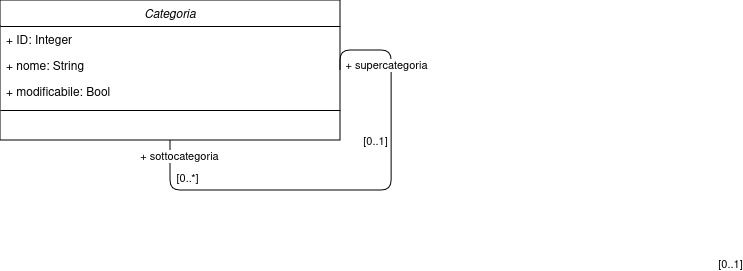
\includegraphics[width=0.5\textwidth]{Images/Categoria-Class.png}
    \caption{Classe Categoria}
    \label{fig:categoria}
\end{figure}

La classe "Categoria" rappresenta le categorie di eventi presenti sul sistema, definibili dagli utenti autorizzati dal comune di Trento.\\

\textbf{Attributi:}\\
Gli attributi che caratterizzano questa classe sono:
\begin{itemize}
    \item \textbf{ID}: Attributo che identifica univocamente la categoria di eventi.
    \item \textbf{nome}: Attributo che rappresenta il nome della categoria di eventi.
    \item \textbf{modificabile}: Attributo che rappresenta lo stato di modificabilità della categoria.\\
\end{itemize}
Per la classe in questione non sono previsti metodi.

\clearpage

\begin{figure}[htbp]
    \centering
    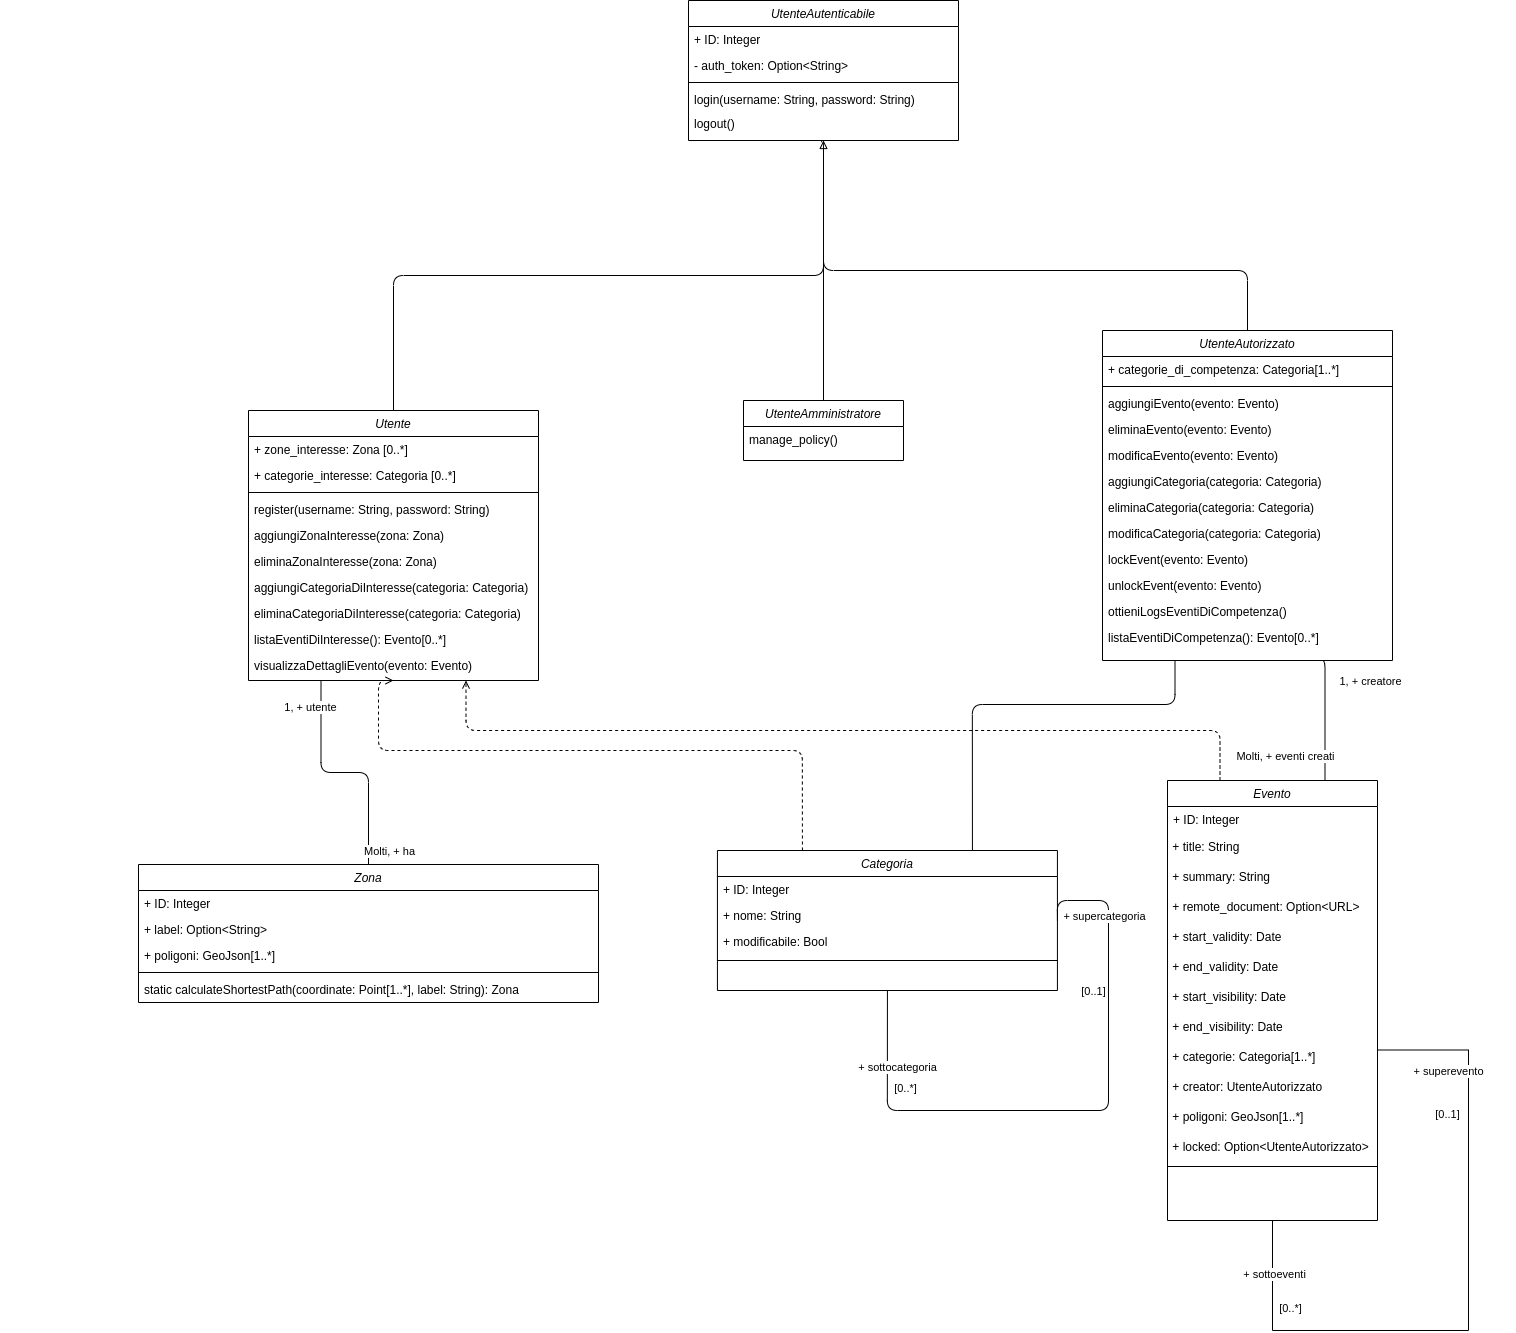
\includegraphics[width=1\textwidth]{Images/ClassDiagram.png}
    \caption{Diagramma delle classi}
    \label{fig:class-diagram}
\end{figure}
